\documentclass[sigplan,10pt]{acmart}

\usepackage[T1]{fontenc}
\usepackage[utf8]{inputenc}

\usepackage{acronym} % \ac[p], \acl[p], \acs[p], \acf[p]
\usepackage{algorithm} % \begin{algorithm} \end{algorithm}
\usepackage{algpseudocode} % \begin{algorithmic} \end{algorithmic}
\usepackage[inline]{enumitem} % \begin{enumerate*} \end{enumerate*}

\usepackage{graphicx}
\usepackage{color}
\AtBeginDocument{
\definecolor{pdfurlcolor}{rgb}{0,0,0}
\definecolor{pdfcitecolor}{rgb}{0,0,0}
\definecolor{pdflinkcolor}{rgb}{0,0,0}
\definecolor{light}{gray}{.85}
\definecolor{vlight}{gray}{.95}
\definecolor{darkgreen}{rgb}{0.0, 0.2, 0.13}
}

\usepackage[draft,inline,nomargin,index]{fixme}
\fxsetup{theme=colorsig,mode=multiuser,inlineface=\itshape,envface=\itshape}
\FXRegisterAuthor{go}{ago}{Gerald}
\FXRegisterAuthor{mn}{amn}{Matthieu}

\usepackage{subcaption} % subfigure

\def\algorithmautorefname{Algorithm}

% Commands
%---------
\newcommand{\inbb}[1]{\in \mathbb{#1}}
\newcommand{\mathlist}[2]{\set{#1_i \in #2}_{i \inbb{N}}}
\newcommand{\set}[1]{\left\{#1\right\}} % set brace notation

% Acronyms
% --------
\acrodef{ADT}[ADT]{Abstract Data Type}
\acrodefplural{ADT}[ADTs]{Abstract Data Types}

\acrodef{CRDT}[CRDT]{Conflict-free Replicated Data Type}
\acrodefplural{CRDT}[CRDTs]{Conflict-free Replicated Data Types}

\acrodef{JIT}[JIT]{Just-In-Time}

\acrodef{OT}[OT]{Operational Transform}

\acrodef{P2P}[P2P]{Peer-to-Peer}

\acrodef{SEC}[SEC]{Strong Eventual Consistency}

\begin{document}

\title{Efficient Renaming in \acp{CRDT}}

\author{Matthieu Nicolas}
\email{matthieu.nicolas@loria.fr}
\affiliation{%
  \institution{Université de Lorraine, CNRS, Inria, LORIA, F-54500}
  \city{Nancy}
  \country{France}
}

\author{Gérald Oster}
\email{gerald.oster@loria.fr}
\affiliation{%
  \institution{Université de Lorraine, CNRS, Inria, LORIA, F-54500}
  \city{Nancy}
  \country{France}
}

\author{Olivier Perrin}
\email{olivier.perrin@loria.fr}
\affiliation{%
  \institution{Université de Lorraine, CNRS, Inria, LORIA, F-54500}
  \city{Nancy}
  \country{France}
}

\begin{abstract}
To achieve high availability, large-scale distributed systems have to replicate data and to minimise coordination between nodes. The literature and industry increasingly adopt Conflict-free Replicated Data Types (CRDTs) to design such systems. CRDTs are data types which behave as traditional ones, e.g. the Set or the Sequence. However, compared to traditional data types, they are designed to support natively concurrent modifications. To this end, they embed in their specification a conflict-resolution mechanism.

To resolve conflicts in a deterministic manner, CRDTs usually attach identifiers to elements stored in the data structure. Identifiers have to comply with several constraints such as uniqueness or being densely ordered according to the kind of CRDT. These constraints may prevent the identifiers’ size from being bounded. As the number of the updates increases, the size of identifiers grows. This leads to performance issues, since the efficiency of the replicated data structure decreases over time.

To address this issue, we propose a new CRDT for Sequence which embeds a renaming mechanism. It enables nodes to reassign shorter identifiers to elements in an uncoordinated manner. Obtained experiment results demonstrate that this mechanism decreases the overhead of the replicated data structure and eventually limits it.
\end{abstract}

\keywords{CRDT, collaborative editing}

\maketitle

\section{Introduction}

\begin{itemize}
    \item Real-time collaborative text editing
    \item \ac{OT}
    \item \ac{CRDT}
\end{itemize}

\section{Background}

To solve conflicts deterministically and ensure the convergence of all nodes, \acp{CRDT} relies on additional metadata.
In the context of Sequence \acp{CRDT}, two different approaches were proposed, each trying to minimize the overhead introduced.
The first one affixes constant-sized identifiers to each value in the sequence and uses them to represent the sequence as a linked list.
The downside of this approach is an evergrowing overhead, as it needs to keep removed values to deal with potential concurrent updates, effectively turning them into tombstones.
The second one avoids the need of tombstones by instead attaching densely-ordered identifiers to values.
It is then able to order values into the sequence by comparing their respective identifiers.
However this approach also suffers from an ever-increasing overhead, as the size of such densely-ordered identifiers is variable and grows over time.

In the context of this paper, we focus on the later approach.

\subsection{LogootSplit}

\begin{itemize}
    \item Attach dense identifiers to elements
    \item Group elements with adjacent identifiers into blocks to reduce overhead
\end{itemize}

\subsection{Limits}

\begin{itemize}
    \item Growth of identifiers
    \item Increasing number of blocks
\end{itemize}

\section{Proposed approach}

We propose a new Sequence \ac{CRDT} relying on dense identifiers to order elements : \emph{RenamableLogootSplit}.

To address the limitations of LogootSplit, we embed in this data structure a renaming mechanism.
The purpose of this mechanism is to reassign shorter identifiers to values in such a manner that we are then able to aggregate them into one unique block.
This allows to reduce the metadata of the whole sequence.
However, as the goal is to reduce LogootSplit's evergrowing memory overhead, we have to design the renaming mechanism while minimizing its own footprint.

\subsection{\emph{rename} operation}

\begin{itemize}
    \item Reassign arbitrary identifiers to elements
    \item Such as elements can be grouped into only one block, independently of the current size of the sequence
\end{itemize}

\subsection{Dealing with concurrent updates}

\label{sec:dealing-with-concurrent-updates}

\begin{itemize}
    \item Applying it as such would lead to inconsistencies
    \item Need to detect concurrent updates
    \item Set epoch-based system
    \begin{itemize}
        \item Each \emph{rename} operation makes sequence move to new epoch
        \item Attach to operations epoch of generation
    \end{itemize}
    \item Need to transform concurrent updates
    \item Add rewriting rules
    \begin{itemize}
        \item Find id of predecessor in former state
        \item Compute its counterpart in renamed state
        \item Use it as a prefix
    \end{itemize}
\end{itemize}

As \emph{rename} operations can be issued without any kind of coordination, it is possible for other nodes to perform concurrent updates.

\subsection{Downsides}

\begin{itemize}
    \item Need to store former until no more concurrent operations
    \item Need to broadcast former state to other nodes
\end{itemize}

\section{Evaluation}

\subsection{Simulations and benchmarks}

To validate the proposed renaming mechanism, we performed an experimental evaluation to measure its performances on several aspects:
\begin{enumerate*}
    \item the size of the data structure
    \item the integration time of the \emph{rename} operation
    \item the integration time of \emph{insert} and \emph{remove} operations.
\end{enumerate*} In cases 1 and 3, we use LogootSplit as the baseline data structure to compare results.

Since we were not able to retrieve an existing dataset of traces of realtime collaborative editing sessions, we ran simulations to generate traces to evaluate our data structure.
The simulations depict the following scenario: several authors collaborate in order to write an article.
Initially, they prioritize adding content as everything remains to be done.
Thus they mainly insert elements into the document during this first phase.
A few \emph{remove} operations are still issued to simulate spelling mistakes.
Once the document approaches the critical length, the collaborators switch to the second phase.
From this point, they stop adding new content and focus on revamping existing parts instead.
This is simulated by balancing the ratio between \emph{insert} and \emph{remove} operations.
Each author has to perform a given number of operations and the collaboration ends once every all of them received all operations.
We take snapshots of the document at given steps of the collaboration to follow the evolution of the document.

We ran these simulations with the following experimental settings : we deployed 10 bots as separate Docker containers on a single workstation.
Each container corresponds to a single mono-threaded Node.js process (version 13.1.0) simulating an author.
The bots share and edit collaboratively the document using either LogootSplit or RenamableLogootSplit according to the session.
In both cases, each bot performs an \emph{insert} or a \emph{remove} operation locally every 200 $\pm$ 50ms.
During the first phase, the probabilities for each operation of being an \emph{insert} or a \emph{remove} are respectively of 80\% and 20\%.
Once the document reaches 60k characters (around 15 pages), the probabilities are both set to 50\%.
The generated operation is then broadcast to others using a \ac{P2P} full mesh network.
After issuing an operation, there are 5\% of chances that the bot moves its cursor to another position in the document.
Each bot performs 15k operations.
Snapshots are taken every 10k operations overall.
Additionally, in the case of RenamableLogootSplit, one bot is arbitrarily designated as the master.
It performs \emph{rename} operations every 30k operations overall.

The code of the simulations is available at the following address: \url{https://github.com/coast-team/mute-bot-random/}.
This repository also contains the code corresponding to the benchmarks described in the next subsections as well as the results computed.

Meanwhile, our implementation of LogootSplit and RenamableLogootSplit are available at \url{https://github.com/coast-team/mute-structs}.
Both implementations use an AVL Tree, a self-balancing binary search tree, to represent the sequence.
This data structure enables us to achieve \emph{insert} and \emph{remove} operations in logarithmic time.

\subsection{Results}

\paragraph{Memory overhead}

Using the snapshots generated, we compare the evolution of the size of the data structure in collaborative editing session.
The results are displayed in \autoref{fig:evolution-document-size}.
On this plot, the blue line corresponds to the size of the content while the red one exhibits the growth of the LogootSplit data structure.

\begin{figure}
    \centering
    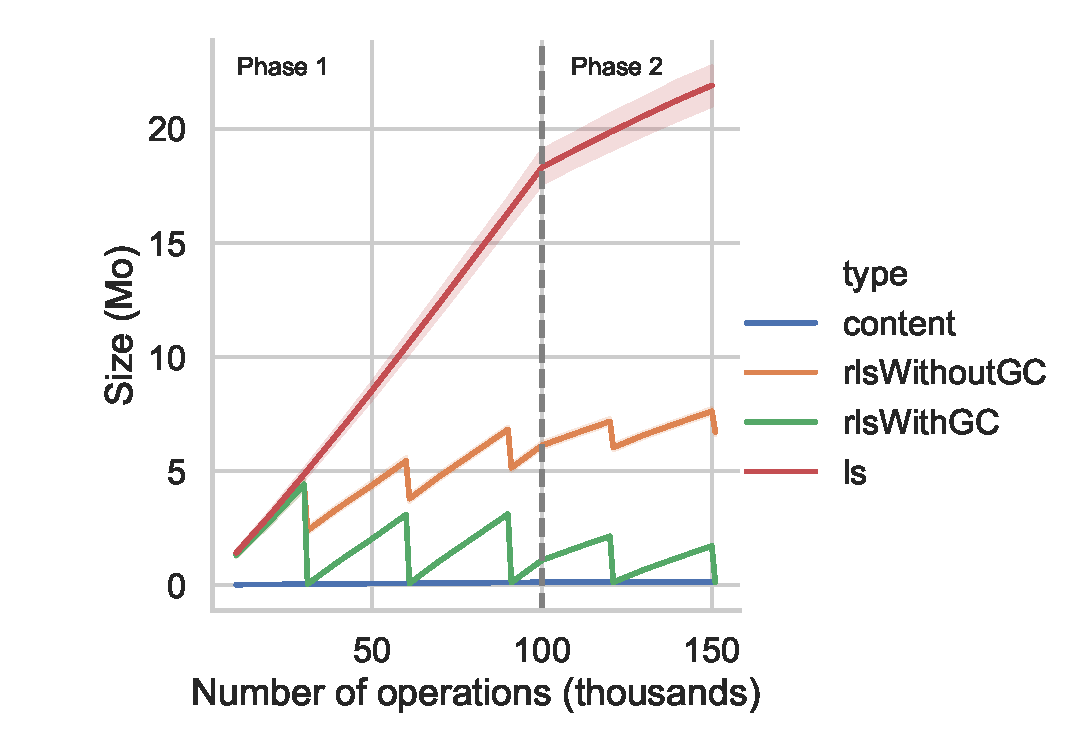
\includegraphics[width=0.5\textwidth]{img/snapshots-sizes.pdf}
    \caption{Evolution of the size of the document}
    \label{fig:evolution-document-size}
\end{figure}

The green line illustrates the growth of the RenamableLogootSplit document in its best-case scenario.
In this scenario, \emph{rename} operations become stable as soon as they are issued.
Former states can then be garbage collected safely, maximizing the benefits of the \emph{renaming} mechanism.
In this case, we observe that \emph{rename} operations reset the overhead of the data structure and eventually reduce by hundred times the document size compared to LogootSplit equivalent one.

As for the orange line, it represents RenamableLogootSplit worst-case scenario.
Here, we assume that \emph{rename} operations never become stable and that nodes has to store former states forever.
However, obtained results show that RenamableLogootSplit outperforms LogootSplit and reduce by 66\% the size of the data structure, even in this case.
This outcome is explained by the fact that the AVL does not only store the content and blocks corresponding to the sequence.
Some metadata is actually added to the state to browse the sequence more efficiently when performing updates.
When a \emph{rename} operation is applied, nodes only keep the sequence of blocks from the former state as an array to be able to transform concurrent operations.
Other metadata is scrapped, which results in this memory gain.

\paragraph{Integration times of standard operations}

We set up benchmarks to measure the impact of the renaming mechanism on the integration times of \emph{insert} and \emph{remove} operations.
The obtained results are presented in \autoref{fig:evolution-integration-time-insert-remove}.

\begin{figure}
    \centering
    \begin{subfigure}{0.35\textwidth}
        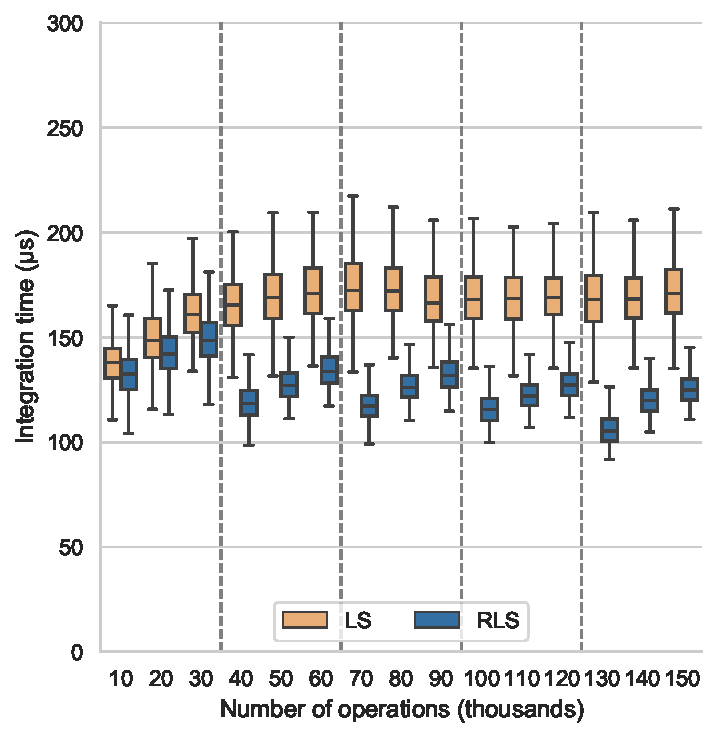
\includegraphics[width=1\textwidth]{img/integration-time-boxplot-local-operations-without-outliers.pdf}
        \caption{Local operations}
        \label{fig:evolution-integration-time-local-insert-remove}
    \end{subfigure}
    \begin{subfigure}{0.35\textwidth}
        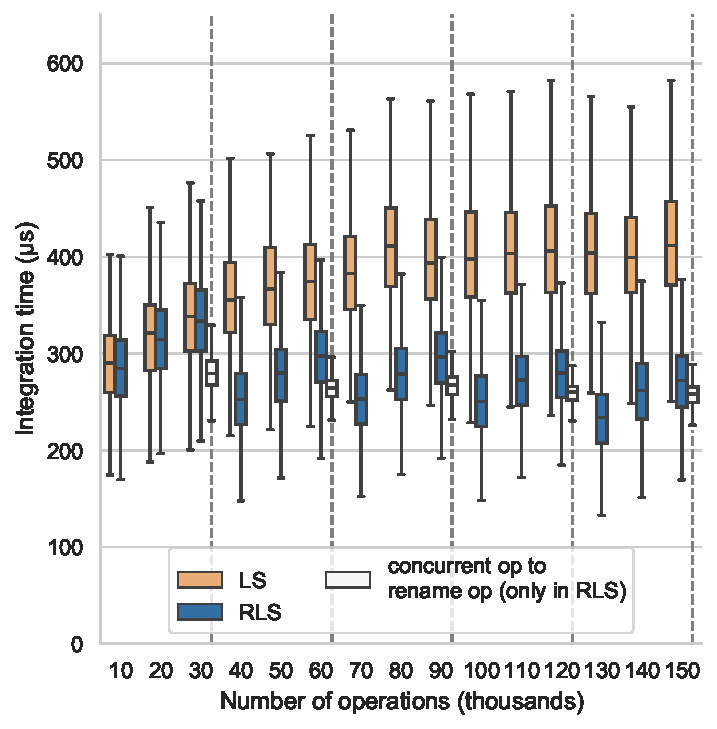
\includegraphics[width=1\textwidth]{img/integration-time-boxplot-remote-operations-without-outliers.pdf}
        \caption{Remote operations}
        \label{fig:evolution-integration-time-remote-insert-remove}
    \end{subfigure}
    \caption{Evolution of the integration time of standard operations}
    \label{fig:evolution-integration-time-insert-remove}
\end{figure}

\autoref{fig:evolution-integration-time-local-insert-remove} displays the integration times of local operations while \autoref{fig:evolution-integration-time-remote-insert-remove} exhibits remote ones.
In both cases, the orange boxplots correspond to LogootSplit's integration times while blue ones to RenamableLogootSplit's ones.
The results show that the \emph{renaming} mechanism allows to reduce the integration times of future operations.

In \autoref{fig:evolution-integration-time-remote-insert-remove}, the green boxplots display the integration times of concurrent operations to a \emph{rename} one.
As illustrated in \autoref{sec:dealing-with-concurrent-updates}, these operations require to be transformed before being applied to the renamed state.
The results presented here show that this is actually faster than applying them directly on the former state.

\paragraph{Integration time of \emph{rename} operation}

Finally, we measured the integration time of the \emph{rename} operation according to the size of the document.
Results are displayed in \autoref{fig:evolution-integration-time-rename}.
In this figure, the blue line corresponds to the integration time of a \emph{local} rename operation while the orange one corresponds to the integration time of a remote one.

\begin{figure}
    \centering
    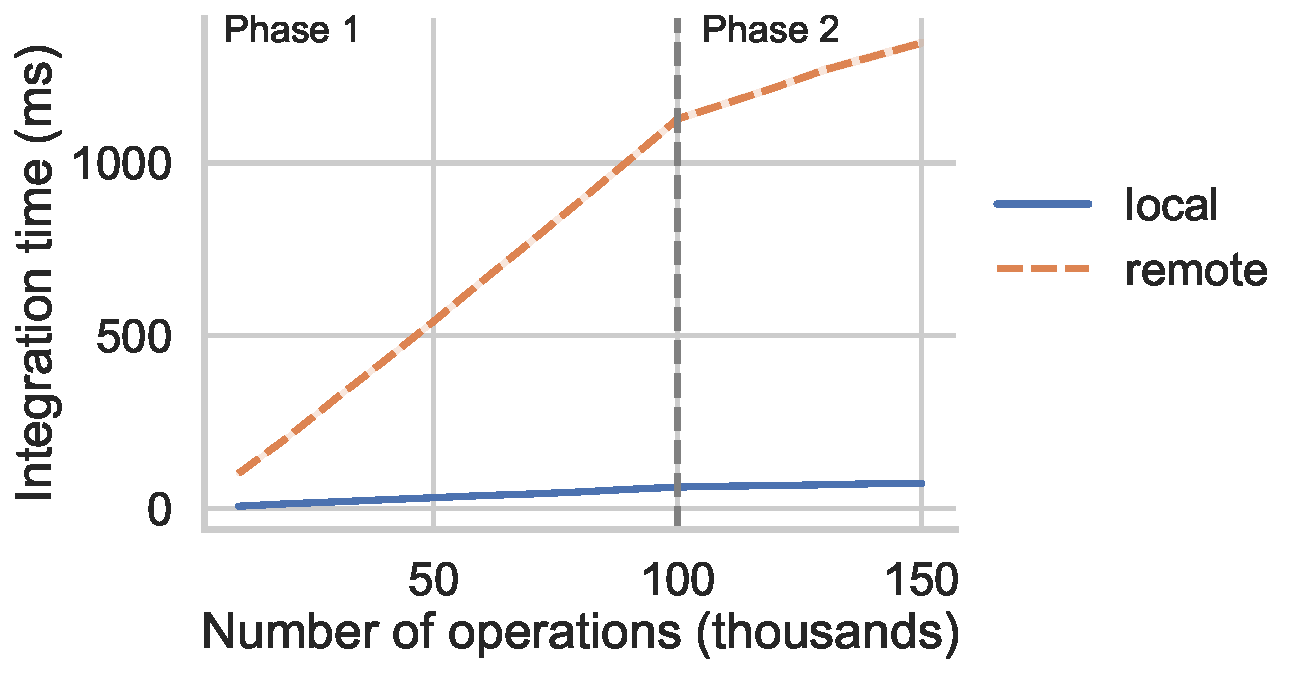
\includegraphics[width=0.5\textwidth]{img/integration-time-rename.pdf}
    \caption{Evolution of the integration time of rename operations}
    \label{fig:evolution-integration-time-rename}
\end{figure}

The main result of this benchmark is that the unit of time used when applying \emph{rename} operations is in hundreds of milliseconds.
However other operations can not be integrated during the processing of \emph{rename} operations : remote operations won't be displayed to the user while local ones won't be propagated to others.
\emph{Rename} operations can thus be perceived as spikes of latency by users and degrade their experience if they are too long to process.
It is necessary to take this concern into account when designing the strategy used to trigger \emph{rename} operations to avoid such cases.


\section{Conclusions and future work}

\end{document}
